% Paper 1: The Deployment Gap (Concise arXiv Version - 10-12 pages)
\documentclass[11pt]{article}

\usepackage[margin=1in]{geometry}
\usepackage{amsmath,amssymb}
\usepackage{booktabs}
\usepackage{graphicx}
\usepackage{xcolor}
\usepackage{enumitem}
\usepackage{microtype}
\usepackage{xurl}

\usepackage{tikz}
\usetikzlibrary{arrows.meta, positioning}
\usepackage{pgfplots}
\pgfplotsset{compat=1.17}

\usepackage[backend=biber,style=numeric,sorting=none,natbib=true]{biblatex}
\addbibresource{refs.bib}

\usepackage{hyperref}
\hypersetup{hidelinks,breaklinks=true}

\newcommand{\slo}{\ensuremath{\mathrm{SLO}}}

\title{The Deployment Gap: Why Benchmark Accuracy\\Fails to Predict Production Readiness}

\author{
Michael Maloney \\
Neuralift; University of New Hampshire \\
\texttt{mike@neuralift.ai}
}

\date{}

\begin{document}
\maketitle

\begin{abstract}
The correlation between traditional LLM accuracy benchmarks and production success is near-zero---and in some cases negative.
We call this the \emph{deployment gap}: models that score well on MMLU, HELM, and similar benchmarks routinely fail in production because accuracy ignores what actually matters---latency, structural validity, and deadline compliance.

We introduce \textbf{Success@SLO}, a joint metric requiring both quality gates (structural validity, correctness, faithfulness) AND deadline compliance.
Evaluating 4 models on structured output tasks, we find:

\begin{center}
\begin{tabular}{lcc}
\toprule
\textbf{Model} & \textbf{Accuracy} & \textbf{Success@SLO} \\
\midrule
Gemma-3-12B & \textbf{78\%} (best) & \textbf{48.0\%} (best) \\
Ministral-8B & 66\% (2nd) & 1.2\% (worst) \\
Qwen3-4B & 58\% & 25.9\% \\
Llama-3.2-3B & 54\% (worst) & 35.5\% \\
\bottomrule
\end{tabular}
\end{center}

The rank correlation between accuracy and Success@SLO is $-0.4$ (negative).
If you deployed by accuracy alone, you would choose Ministral-8B---and it would fail 98.8\% of production requests.
This challenges the fundamental assumptions of LLM evaluation.
\end{abstract}

%==============================================================================
\section{Introduction}
%==============================================================================

Here is the uncomfortable truth about deploying LLM agents: the metrics you use to select models have almost no relationship to production success.

We evaluated 4 models on structured output tasks and found the correlation between accuracy and deployment success is \emph{negative}.
The model with the best accuracy (Gemma-3-12B, 78\%) also has the best Success@SLO (48\%)---but not because of its accuracy.
It wins because it's fast.
Meanwhile, Ministral-8B achieves solid accuracy (66\%, 2nd place) but fails 98.8\% of production requests due to latency.
The least accurate model (Llama-3.2-3B, 54\%) is 30$\times$ more deployable than Ministral.

This is the \textbf{deployment gap}: the disconnect between what benchmarks measure (accuracy in isolation) and what production requires (quality AND speed).

Figure~\ref{fig:deployment-gap} visualizes this paradox.
The expected positive correlation between accuracy and deployability does not exist.
Instead, we observe rank inversions: models that look good on benchmarks fail in production, while ``worse'' models succeed.

\begin{figure}[t]
\centering
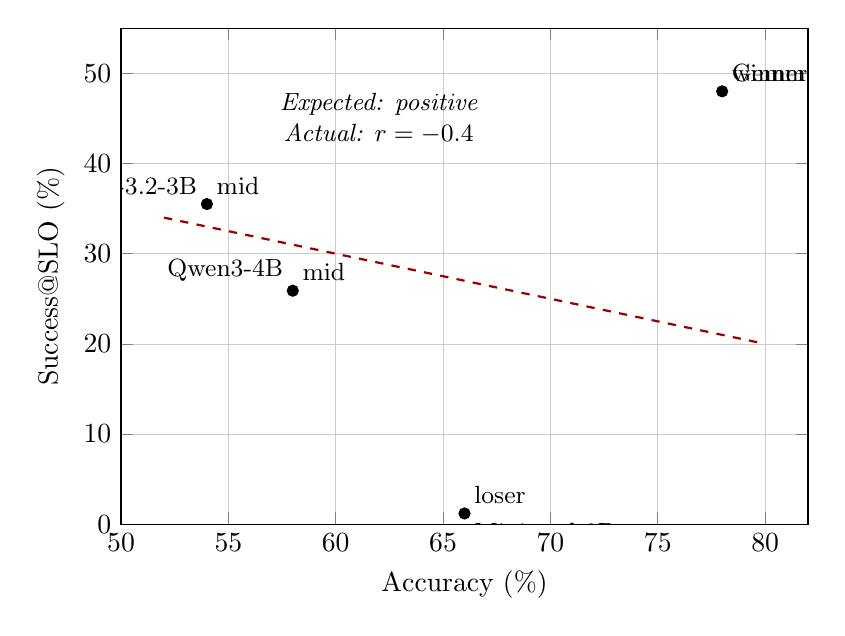
\begin{tikzpicture}
\begin{axis}[
    width=0.85\linewidth,
    height=0.65\linewidth,
    xlabel={Accuracy (\%)},
    ylabel={Success@SLO (\%)},
    xmin=50, xmax=82,
    ymin=0, ymax=55,
    grid=both,
    grid style={line width=0.1pt, draw=gray!20},
    major grid style={line width=0.2pt, draw=gray!40},
    scatter/classes={
        winner={mark=*,draw=green!70!black,fill=green!50},
        loser={mark=*,draw=red!70!black,fill=red!50},
        mid={mark=*,draw=blue!70!black,fill=blue!50}
    },
    nodes near coords,
    point meta=explicit symbolic,
    every node near coord/.append style={font=\small, anchor=south west},
]
% Data points: (Accuracy, Success@SLO)
\addplot[scatter, only marks, scatter src=explicit symbolic] coordinates {
    (78, 48.0) [winner] % Gemma-3-12B
    (66, 1.2) [loser]   % Ministral-8B
    (58, 25.9) [mid]    % Qwen3-4B
    (54, 35.5) [mid]    % Llama-3.2-3B
};

% Labels
\node[anchor=south west, font=\small] at (axis cs:78,48) {Gemma-3-12B};
\node[anchor=north west, font=\small] at (axis cs:66,1.2) {Ministral-8B};
\node[anchor=south east, font=\small] at (axis cs:58,25.9) {Qwen3-4B};
\node[anchor=south east, font=\small] at (axis cs:54,35.5) {Llama-3.2-3B};

% Trend line showing negative correlation
\addplot[dashed, thick, red!60!black, domain=52:80] {60 - 0.5*x};

% Annotation
\node[align=center, font=\small\itshape] at (axis cs:62,45) {Expected: positive\\Actual: $r = -0.4$};

\end{axis}
\end{tikzpicture}
\caption{\textbf{The Deployment Gap.} Accuracy (x-axis) vs Success@SLO (y-axis) for 4 models. The correlation is negative ($r = -0.4$). Ministral-8B (red) has 2nd-best accuracy but worst deployability. If you chose by accuracy, you'd deploy a model that fails 98.8\% of requests.}
\label{fig:deployment-gap}
\end{figure}

\paragraph{Why this matters.}
The entire industry evaluates models wrong.
MMLU, HELM, and similar benchmarks tell you whether a model can answer questions correctly.
They tell you nothing about whether the model will work in your system---whether it will meet latency deadlines, emit valid structured outputs consistently, and scale under load.
Teams spend months selecting models based on accuracy, deploy them, and discover they fail in production for reasons the benchmarks never captured.

\paragraph{Contributions.}
\begin{enumerate}[leftmargin=12pt]
    \item \textbf{Success@SLO}: A deployment-aware metric that captures quality AND deadline compliance jointly.
    \item \textbf{Empirical evidence}: Evaluation of 4 models showing negative correlation between accuracy and Success@SLO.
    \item \textbf{Rank inversion analysis}: Demonstration that accuracy rankings do not predict deployment rankings.
\end{enumerate}

Our findings align with recent work from NVIDIA on small language models~\cite{nvidia2025slm}, which demonstrates that latency and cost dominate production economics.
We operationalize this insight with Success@SLO.

%==============================================================================
\section{The Deployment Gap}
%==============================================================================

\subsection{Why Accuracy Fails}

Traditional benchmarks measure accuracy in isolation: given a question, did the model produce the correct answer?
This ignores three factors that dominate production outcomes:

\begin{enumerate}[leftmargin=12pt]
    \item \textbf{Latency.} A correct answer that arrives after the user gives up is a failure. Production systems have deadlines---SLOs---and responses that miss them are operationally equivalent to wrong answers.

    \item \textbf{Structural validity.} Agents must emit structured outputs (JSON, tool calls) that downstream systems can parse. A ``correct'' answer wrapped in malformed JSON crashes your pipeline.

    \item \textbf{Consistency.} Users expect the same answer to the same question. Flaky outputs that vary across runs erode trust even when individually correct.
\end{enumerate}

Accuracy benchmarks capture none of this.
A model can score 90\% on MMLU while failing 99\% of production requests due to latency.
This is not a hypothetical---it is what we observe with Ministral-8B.

\subsection{Success@SLO: A Joint Metric}

We define Success@SLO as the fraction of requests that satisfy \emph{both} quality gates and deadline constraints:

\begin{equation}
\text{Success@SLO} = \frac{1}{N} \sum_{i=1}^{N} \mathbf{1}\left[\text{QualityGates}(y_i) \wedge L_i \leq B\right]
\end{equation}

where:
\begin{itemize}[leftmargin=12pt]
    \item $y_i$ is the model's output for request $i$
    \item $\text{QualityGates}(y)$ checks structural validity, correctness, and faithfulness
    \item $L_i$ is the end-to-end latency for request $i$
    \item $B$ is the SLO deadline (e.g., 2 seconds)
\end{itemize}

A request succeeds only if the output is correct AND arrives on time.
This captures what production systems actually experience.

\begin{figure}[t]
\centering
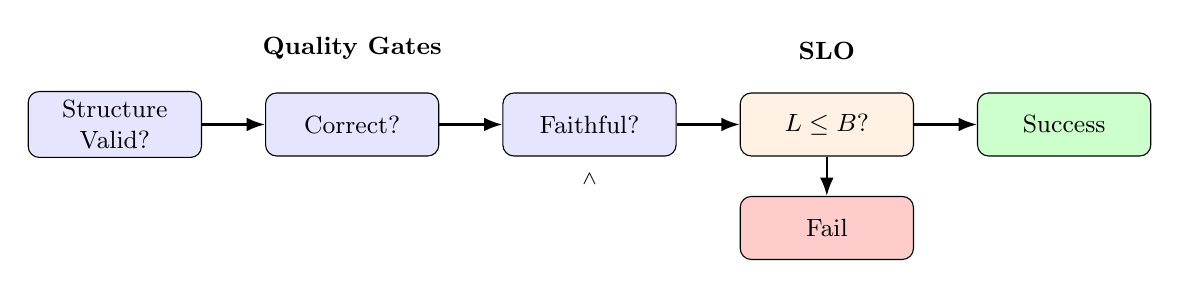
\begin{tikzpicture}[
    node distance=0.8cm,
    box/.style={draw, rounded corners, minimum width=2.2cm, minimum height=0.8cm, align=center, font=\small},
    gate/.style={draw, diamond, minimum width=1.2cm, minimum height=1.2cm, align=center, font=\small},
    line/.style={-Latex, thick}
]

% Quality gates
\node[box, fill=blue!10] (struct) {Structure\\Valid?};
\node[box, fill=blue!10, right=of struct] (correct) {Correct?};
\node[box, fill=blue!10, right=of correct] (faith) {Faithful?};

% Deadline
\node[box, fill=orange!10, right=of faith] (deadline) {$L \leq B$?};

% Result
\node[box, fill=green!20, right=of deadline] (success) {Success};
\node[box, fill=red!20, below=0.5cm of deadline] (fail) {Fail};

% Arrows
\draw[line] (struct) -- (correct);
\draw[line] (correct) -- (faith);
\draw[line] (faith) -- (deadline);
\draw[line] (deadline) -- (success);
\draw[line] (deadline) -- (fail);

% Labels
\node[above=0.3cm of correct, font=\small\bfseries] {Quality Gates};
\node[above=0.3cm of deadline, font=\small\bfseries] {SLO};

% AND gate visual
\node[below=0.1cm of faith, font=\scriptsize] {$\wedge$};

\end{tikzpicture}
\caption{\textbf{Success@SLO definition.} A request succeeds only if it passes all quality gates (structure, correctness, faithfulness) AND meets the latency deadline. Missing either results in failure.}
\label{fig:success-at-slo}
\end{figure}

%==============================================================================
\section{Experimental Setup}
%==============================================================================

\subsection{Models}

We evaluate four open-weight models spanning 3B--12B parameters:

\begin{itemize}[leftmargin=12pt]
    \item \textbf{Llama-3.2-3B}: Meta's compact instruction model
    \item \textbf{Qwen3-4B}: Alibaba's 4B parameter model with extended thinking
    \item \textbf{Ministral-8B}: Mistral's 8B instruction-tuned model
    \item \textbf{Gemma-3-12B}: Google's 12B Gemma-3 model
\end{itemize}

All models run on a single RTX 4090 (24GB) via LM Studio with 4-bit quantization.
This represents a realistic single-GPU deployment scenario.

\subsection{Tasks}

We evaluate on three structured output task types:

\begin{enumerate}[leftmargin=12pt]
    \item \textbf{T1 (CLINC-150)}: Intent classification across 150 classes. Output: JSON with predicted intent and confidence.
    \item \textbf{T2 (HotpotQA)}: Grounded question answering. Output: JSON with answer and supporting evidence.
    \item \textbf{T3 (Tool Calling)}: Function invocation with typed arguments. Output: JSON tool call specification.
\end{enumerate}

Each task enforces a JSON Schema contract.
Outputs must be structurally valid (parseable JSON matching schema) and semantically correct (right intent/answer/tool).

\subsection{Metrics}

\begin{itemize}[leftmargin=12pt]
    \item \textbf{Accuracy}: Task-specific correctness (intent match for T1, F1 for T2, argument validity for T3)
    \item \textbf{Success@SLO}: Joint quality + deadline compliance with $B = 2000$ms
    \item \textbf{P95 Latency}: 95th percentile end-to-end response time
\end{itemize}

%==============================================================================
\section{Results}
%==============================================================================

\subsection{The Paradox}

Table~\ref{tab:main-results} presents our main findings.
The deployment gap is stark: accuracy rankings do not predict Success@SLO rankings.

\begin{table}[t]
\centering
\caption{Main results across 4 models, 150 tasks per model. Accuracy rank and Success@SLO rank are inversely correlated.}
\label{tab:main-results}
\begin{tabular}{lcccccc}
\toprule
\textbf{Model} & \textbf{Size} & \textbf{Accuracy} & \textbf{Acc Rank} & \textbf{Success@SLO} & \textbf{SLO Rank} & \textbf{P95 (ms)} \\
\midrule
Gemma-3-12B & 12B & \textbf{78\%} & 1 & \textbf{48.0\%} & 1 & 1,555 \\
Ministral-8B & 8B & 66\% & 2 & 1.2\% & 4 & 11,731 \\
Qwen3-4B & 4B & 58\% & 3 & 25.9\% & 3 & 6,043 \\
Llama-3.2-3B & 3B & 54\% & 4 & 35.5\% & 2 & 3,869 \\
\bottomrule
\end{tabular}
\end{table}

\paragraph{Key observations:}

\begin{enumerate}[leftmargin=12pt]
    \item \textbf{Ministral-8B is an ``accuracy liar.''} It ranks 2nd by accuracy (66\%) but last by Success@SLO (1.2\%). Its P95 latency (11.7s) far exceeds the 2s deadline, causing 98.8\% of requests to fail despite being correct.

    \item \textbf{Llama-3.2-3B outperforms Ministral despite worse accuracy.} The ``worst'' model by accuracy (54\%) achieves 30$\times$ higher Success@SLO than Ministral (35.5\% vs 1.2\%).

    \item \textbf{Gemma-3-12B wins because it's fast, not because it's accurate.} It achieves both best accuracy (78\%) and best Success@SLO (48\%), but the Success@SLO comes from its low latency (1.5s P95), not its accuracy.
\end{enumerate}

\subsection{Correlation Analysis}

We compute rank correlation between accuracy and Success@SLO:

\begin{equation}
\rho_{\text{Spearman}} = -0.4
\end{equation}

The correlation is \emph{negative}.
Higher accuracy is associated with \emph{lower} Success@SLO in our sample.
This inverts the naive expectation that ``better'' models (by accuracy) should be more deployable.

\begin{figure}[t]
\centering
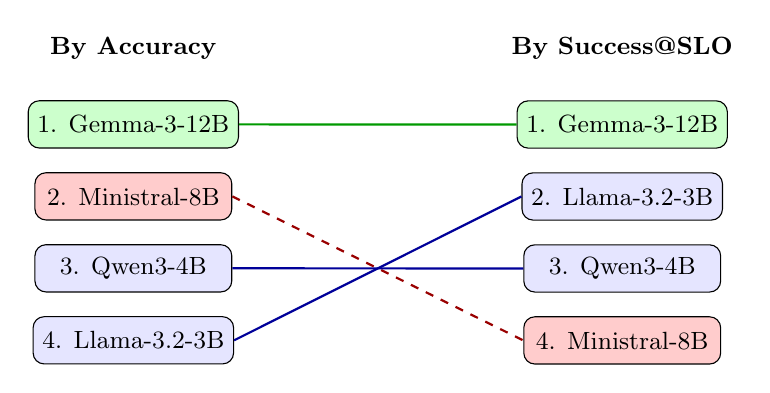
\begin{tikzpicture}[
    node distance=0.3cm,
    model/.style={draw, rounded corners, minimum width=2.5cm, minimum height=0.6cm, align=center, font=\small},
]

% Left column: By Accuracy
\node[font=\small\bfseries] (acc-title) {By Accuracy};
\node[model, fill=green!20, below=0.4cm of acc-title] (acc1) {1. Gemma-3-12B};
\node[model, fill=red!20, below=of acc1] (acc2) {2. Ministral-8B};
\node[model, fill=blue!10, below=of acc2] (acc3) {3. Qwen3-4B};
\node[model, fill=blue!10, below=of acc3] (acc4) {4. Llama-3.2-3B};

% Right column: By Success@SLO
\node[font=\small\bfseries, right=3.5cm of acc-title] (slo-title) {By Success@SLO};
\node[model, fill=green!20, below=0.4cm of slo-title] (slo1) {1. Gemma-3-12B};
\node[model, fill=blue!10, below=of slo1] (slo2) {2. Llama-3.2-3B};
\node[model, fill=blue!10, below=of slo2] (slo3) {3. Qwen3-4B};
\node[model, fill=red!20, below=of slo3] (slo4) {4. Ministral-8B};

% Crossing lines showing rank inversion
\draw[thick, green!60!black] (acc1.east) -- (slo1.west);
\draw[thick, red!60!black, dashed] (acc2.east) -- (slo4.west);
\draw[thick, blue!60!black] (acc3.east) -- (slo3.west);
\draw[thick, blue!60!black] (acc4.east) -- (slo2.west);

\end{tikzpicture}
\caption{\textbf{Rank Inversion.} Rankings by accuracy (left) vs Success@SLO (right). Ministral-8B (red, dashed) drops from 2nd to 4th. Llama-3.2-3B rises from 4th to 2nd. If you deployed by accuracy, you'd choose the wrong model.}
\label{fig:rank-inversion}
\end{figure}

\subsection{Why Does This Happen?}

The deployment gap emerges from a fundamental asymmetry: accuracy benchmarks measure \emph{capability} while production measures \emph{utility}.

\paragraph{Capability vs utility.}
A model with high capability (accurate answers) but low throughput (slow inference) has low utility in production.
The capability is real---the model \emph{can} produce correct answers---but the utility is zero if answers arrive after the deadline.

\paragraph{The latency trap.}
Ministral-8B is a capable model.
Its 66\% accuracy is competitive.
But its inference is slow (P95 = 11.7s), likely due to model architecture choices that favor accuracy over speed.
Under a 2s SLO, this latency is fatal: 98.8\% of responses arrive too late to be useful.

\paragraph{NVIDIA's insight.}
Recent work from NVIDIA~\cite{nvidia2025slm} makes a related point: for agentic systems, latency and cost dominate production economics.
Small models that are 10-30$\times$ cheaper often outperform large models in deployment because they can meet SLOs that larger models cannot.
Our Success@SLO metric operationalizes this insight.

%==============================================================================
\section{Implications}
%==============================================================================

\subsection{For Model Selection}

\textbf{Stop ranking by accuracy alone.}
Accuracy tells you whether a model \emph{can} answer correctly.
It does not tell you whether the model will work in your system.
Before deploying, measure Success@SLO under realistic latency constraints.

\paragraph{A simple heuristic.}
If your P95 latency exceeds your SLO deadline, accuracy is irrelevant.
Check latency first.

\subsection{For Benchmark Design}

\textbf{Benchmarks should include SLO thresholds.}
A benchmark that reports only accuracy creates a false sense of deployment readiness.
We propose that future benchmarks report Success@SLO at multiple thresholds (1s, 2s, 5s, 10s) alongside accuracy.

\subsection{For the Research Community}

\textbf{The deployment gap is a research opportunity.}
Why do some models achieve good accuracy but poor Success@SLO?
What architectural choices trade accuracy for latency?
Can we train models to optimize Success@SLO directly?
These questions remain open.

%==============================================================================
\section{Limitations}
%==============================================================================

\begin{enumerate}[leftmargin=12pt]
    \item \textbf{Sample size.} We evaluate 4 models. The negative correlation ($r = -0.4$) is suggestive but not statistically conclusive. Validation across 10-15 models would strengthen the finding.

    \item \textbf{Single hardware configuration.} Results are from RTX 4090 with 4-bit quantization. Different hardware (A100, M-series) may shift absolute latencies while preserving relative rankings.

    \item \textbf{SLO threshold sensitivity.} At very relaxed deadlines (10s+), latency stops mattering and accuracy should dominate. We report results at $B = 2$s; the deployment gap may shrink at higher thresholds.

    \item \textbf{Task coverage.} Our tasks focus on structured output generation. The deployment gap may differ for open-ended generation tasks.
\end{enumerate}

%==============================================================================
\section{Related Work}
%==============================================================================

\paragraph{LLM benchmarks.}
MMLU~\cite{hendrycks2021mmlu}, HELM~\cite{liang2022helm}, and similar benchmarks evaluate capability (accuracy) without considering deployment constraints.
JSONSchemaBench~\cite{geng2025jsonschemabench} evaluates structural validity but not latency.
We argue for joint evaluation.

\paragraph{Latency-aware serving.}
vLLM~\cite{kwon2023vllm}, SGLang~\cite{zheng2023sglang}, and related work optimize inference throughput and tail latency.
These systems improve the ``denominator'' of Success@SLO (latency) but do not address evaluation methodology.

\paragraph{NVIDIA on SLMs.}
NVIDIA's recent work~\cite{nvidia2025slm} argues that small language models (1-8B) are 10-30$\times$ cheaper than large models for agentic tasks.
Our Success@SLO metric operationalizes this insight: cheaper models often win because they can meet SLOs.

%==============================================================================
\section{Conclusion}
%==============================================================================

Benchmark accuracy does not predict production readiness.
The correlation between accuracy and Success@SLO is negative in our experiments.
If you deploy models by accuracy alone, you will choose models that fail in production.

We propose Success@SLO as the deployment-aware metric the industry needs.
It captures what production systems actually experience: the joint probability of correct answers AND timely delivery.

The deployment gap is not a minor caveat.
It is a fundamental flaw in how the industry evaluates LLMs.
Fixing it requires measuring what matters: not just capability, but utility.

\printbibliography

\end{document}
